% This part is the latex header. It defines what kind of document this will be and 
% says which packages to use. Packages let you include different kind of formats
% and templates in the document. 
\documentclass[11pt]{article} % document type - other options are journal or book?
\usepackage[pdftex]{graphicx} % package to import figures
\usepackage{float} % used for placing figures - H
\usepackage{hyperref} % used for including links (hyper links)
\usepackage{enumerate} % used for making lists
\usepackage[margin=1cm]{geometry}
\usepackage{tabularx}
\usepackage{booktabs}
\usepackage{amsmath}
\usepackage[version=3]{mhchem} 
\usepackage{siunitx}

% math packages
\usepackage{amssymb}
\usepackage{amsmath}

\pagestyle{headings}
\topmargin -0.5in
\oddsidemargin 0.0in
\textwidth 6.5in
\textheight 9.0in

% declare the title, date and author
\title{Radial Bias Pilot 1}
\date{Mar 24, 2021}
\author{Rania Ezzo}

% This is where the actual document starts
\begin{document}
\maketitle
\tableofcontents


\section{Goal of Pilot 1}
To measure radial direction bias with 1D drifting gratings at 8 polar angle locations at 7 deg eccentricity. A total of 3 motion conditions will be tested, 2 radial (inwards and outwards) and 1 tangential (combined), to measure the performance differences between (1) centrifugal and centripetal motion directions, and (2) radial and tangential motion directions. 

\subsection{Parameters}
Eccentricity from central fixation: 7 degrees
\\
Locations tested (polar angle relative to fixation): 0-315 degrees in 45 degree increments
\\
Stimulus: sine wave gratings w/ 0.4 deg sigma gaussian mask
\\
Stimulus spatial frequency: 1 c/deg
\\
Stimulus drift speed: 8 deg/s
\\
Stimulus contrast: full contrast + gaussian mask
\\
Stimulus aperature diameter: 2.5 deg
\\
Black circular aperature was put onto screen to avoid perceptual artifacts from screen edges
\\
Number of subjects: 1-2

\subsection{Experimental Design}
The pilot uses a 2AFC paradigm, within a block each trial includes a drifting grating presented at 1 of 4 possible positions, while the subject maintains fixation at the central dot. A method of constant stimuli is used which is set based on the performance of the training session (see Methods). The angular values added to the internal reference frame is chosen at random from the following constants [-8, -4, -2, -1, -0.5, 0.5, 1, 2, 4, 8] -- logarithmic spacing from 0.5 to 8. The observer must determine whether the direction of motion if clockwise or counterclockwise relative to the internal reference. The sequence of each trial for the 4 motion standards (specific to diagonal locations) at one location is depicted below:

\begin{figure}[H]
\centering % centers the figure
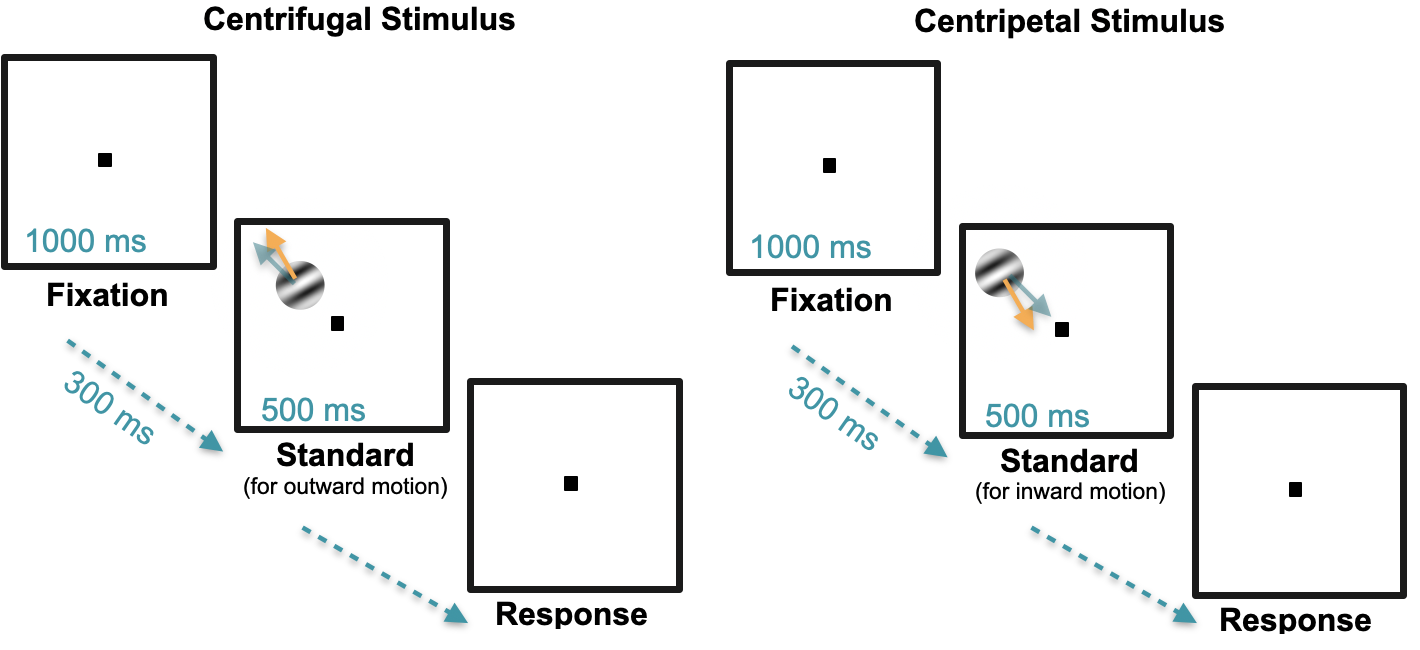
\includegraphics[scale=.4]{Images/Radial_sequence.png}
\\
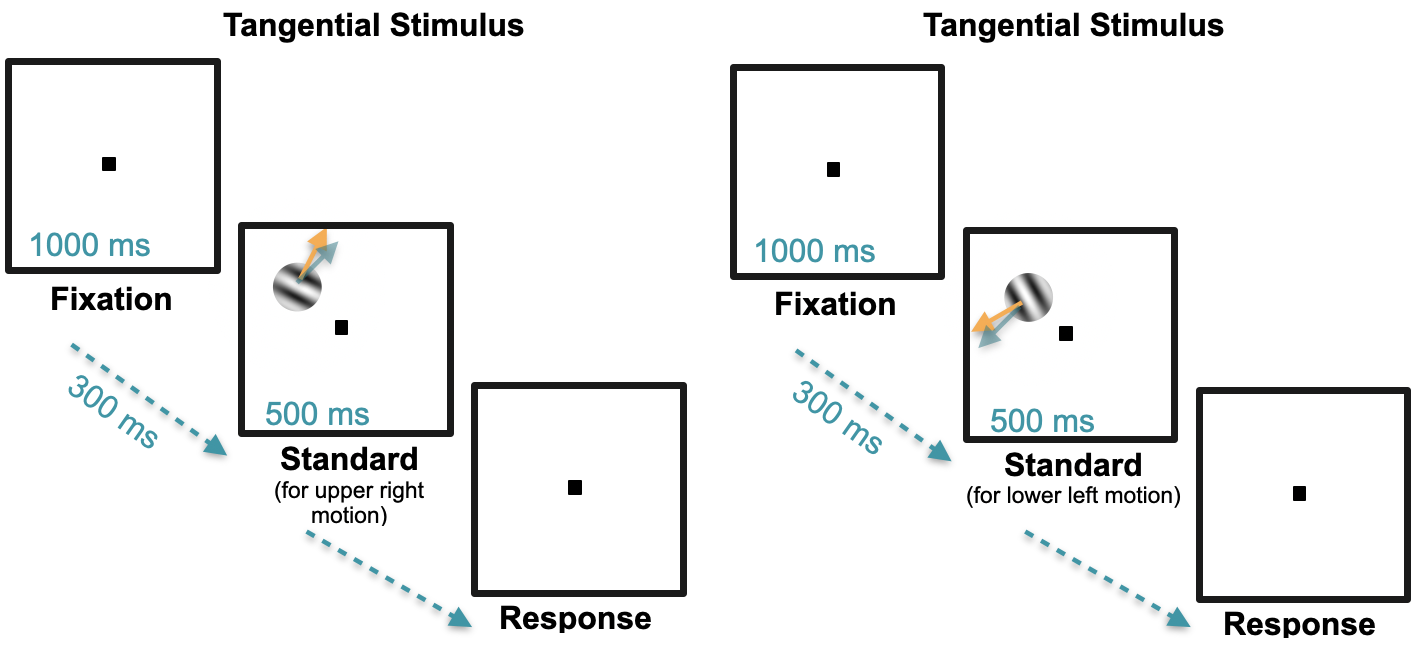
\includegraphics[scale=.4]{Images/Tang_sequence.png}
\caption{Blue arrow represents the internal reference, the orange arrow represents an example of the direction at which the stimulus is presented (can be clockwise or counterclockwise to the blue arrow.}
\end{figure}

\subsection{Block sequence}
Four blocks were run, and each block corresponded to 1 of the 4 conditions being tested (tangential lower left motion, tangential upper right motion, radial upper left motion, radial lower right motion). The internal reference frames for each block is shown below:

\begin{figure}[H]
\centering % centers the figure
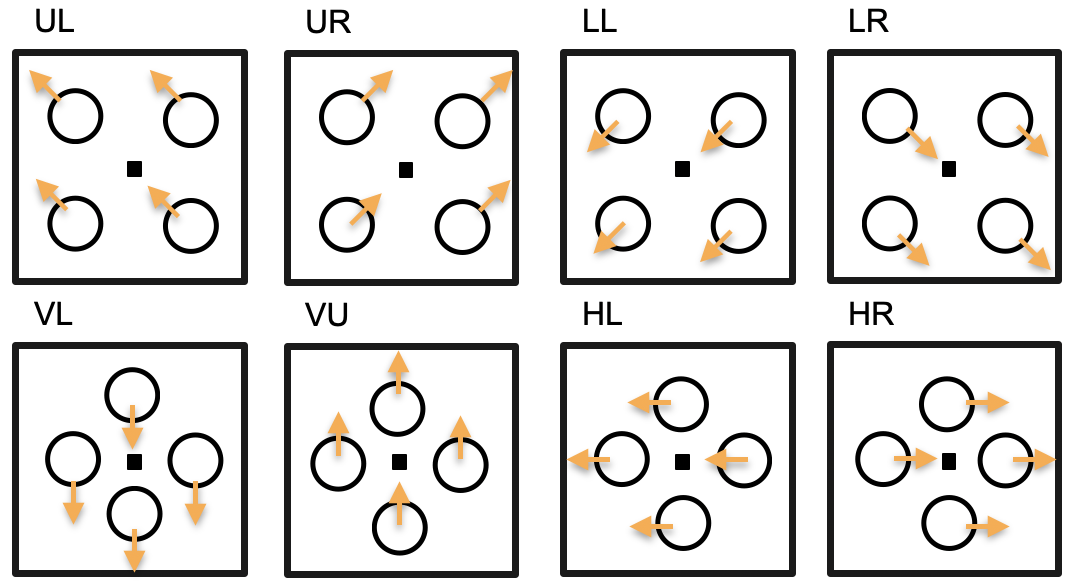
\includegraphics[scale=.4]{Images/Blocks.png}
\end{figure}

Prior to the actual experiment, the "standard" motion direction corresponding to that specific block will be showed to the observer to use as an internal reference. Then a training session is conducted to determine how much tilt is required to meet 75\% accuracy with staircase procedure (MLPest), and to allow subject to practice task with feedback. The estimated angular value to add/subtract to the standard to achieve 75\% performance of the clockwise/counterclockwise will be used to determine constants. For this pilot, constants [-8, -4, -2, -1, -0.5, 0.5, 1, 2, 4, 8] were chosen for all 8 blocks. Note positive and negative values for clockwise v. counterclockwise tilt.
\\
%Each block contains (2 locations with clockwise/counterclockwise motion) x 80 repetitions = 1,280 trials. All 4 full-blocks took 80 min. 
Each block contained 4 locations x 5 tilt values x 2 (clock v cc) x 20 repetitions = 800 trials. There are 8 blocks * 800 trials = 6400 total trials (3200 tang, 1600 radial-in, 1600 radial-out). Each full-block takes ~35 min; all 8 blocks took 280 min. 
\\
RE sequence of blocks 
\begin{enumerate}
\item diag-UL [angles: +- 0.5, 1, 2, 4, 8] (35 min)
\item card-HR [angles: +- 0.5, 1, 2, 4, 8] (35 min)
\item diag-LR [angles: +- 0.5, 1, 2, 4, 8] (35 min)
\item card-VL [angles: +- 0.5, 1, 2, 4, 8] (35 min)
\item diag-UR [angles: +- 0.5, 1, 2, 4, 8] (35 min)
\item card-HL [angles: +- 0.5, 1, 2, 4, 8] (35 min)
\item diag-LL [angles: +- 0.5, 1, 2, 4, 8] (35 min)
\item card-VU [angles: +- 0.5, 1, 2, 4, 8] (35 min)
\end{enumerate}

\newpage
\section{Data}
\subsection{Psychometric Function (Cumulative normal)}
\begin{figure}[H]
\centering % centers the figure
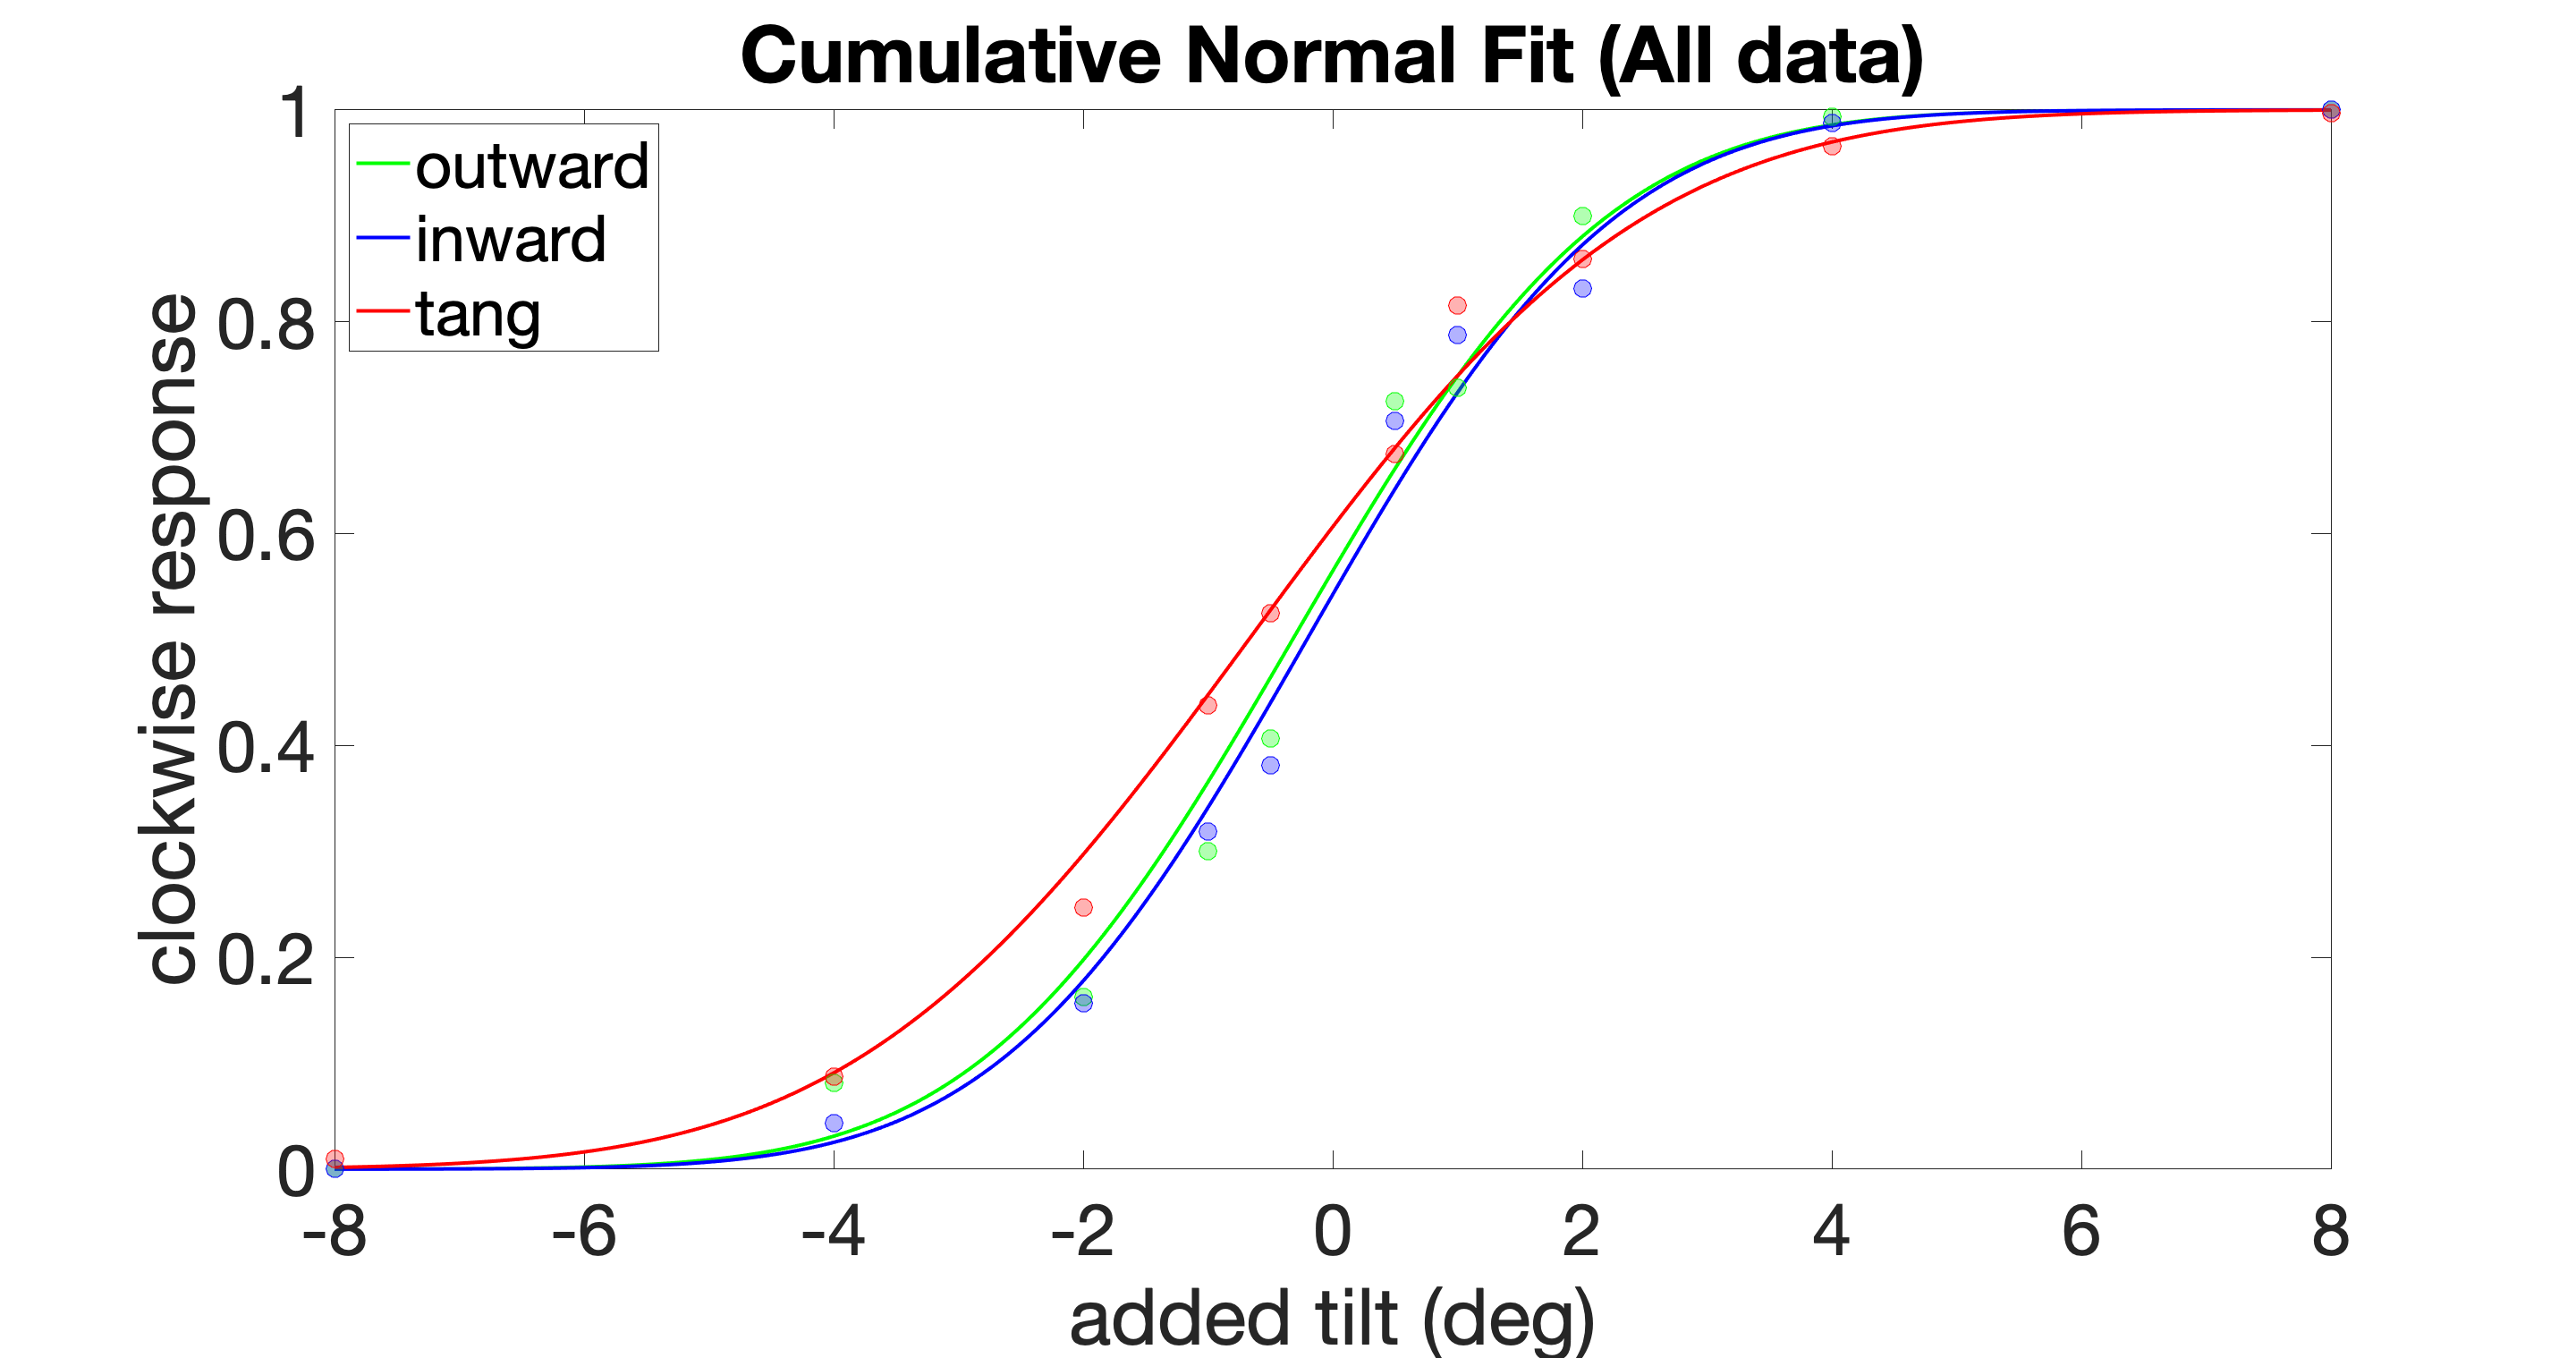
\includegraphics[scale=.06]{Images/PF_cardobl.png}
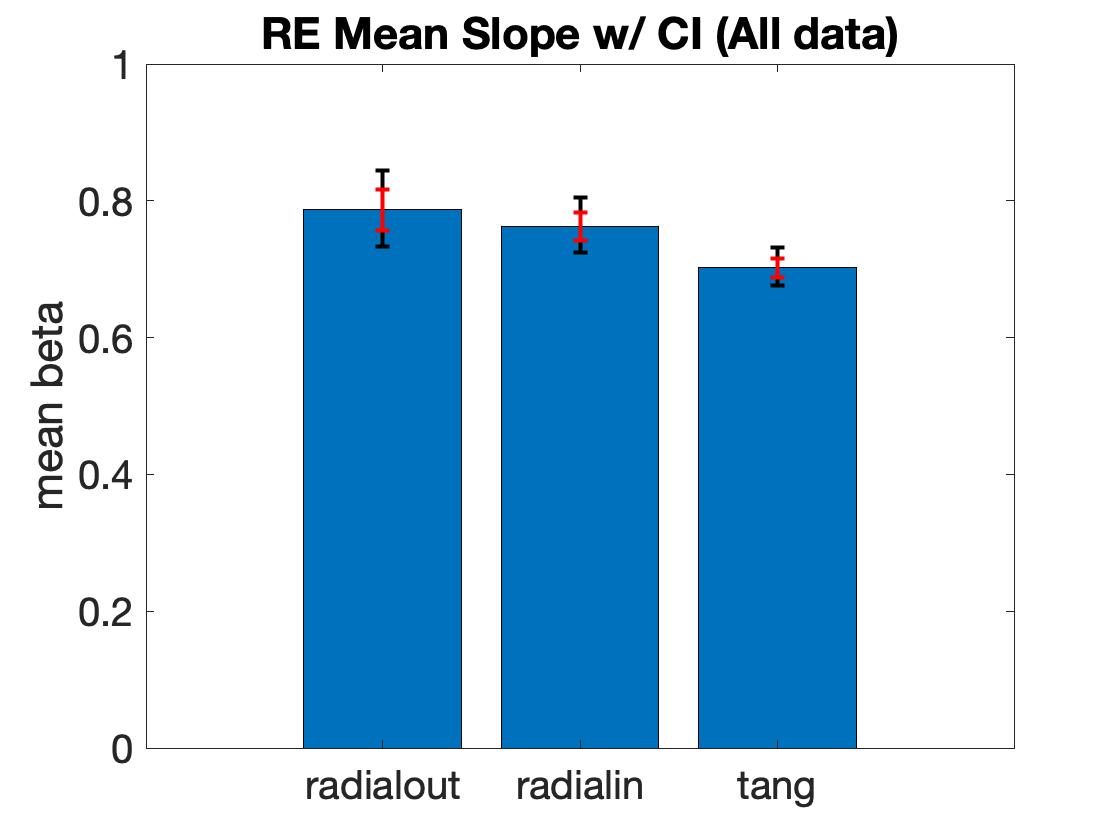
\includegraphics[scale=.11]{Images/MeanSlopeError_cardobl.png}
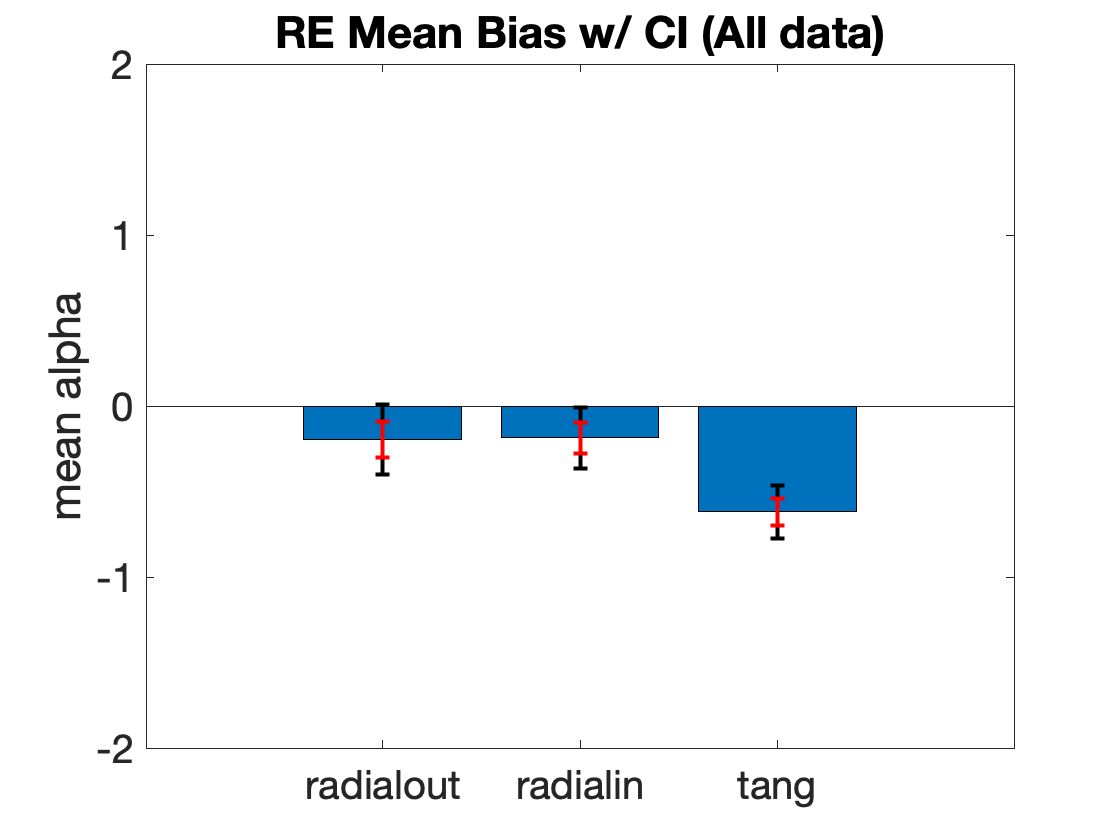
\includegraphics[scale=.11]{Images/MeanBiasError_cardobl.png}
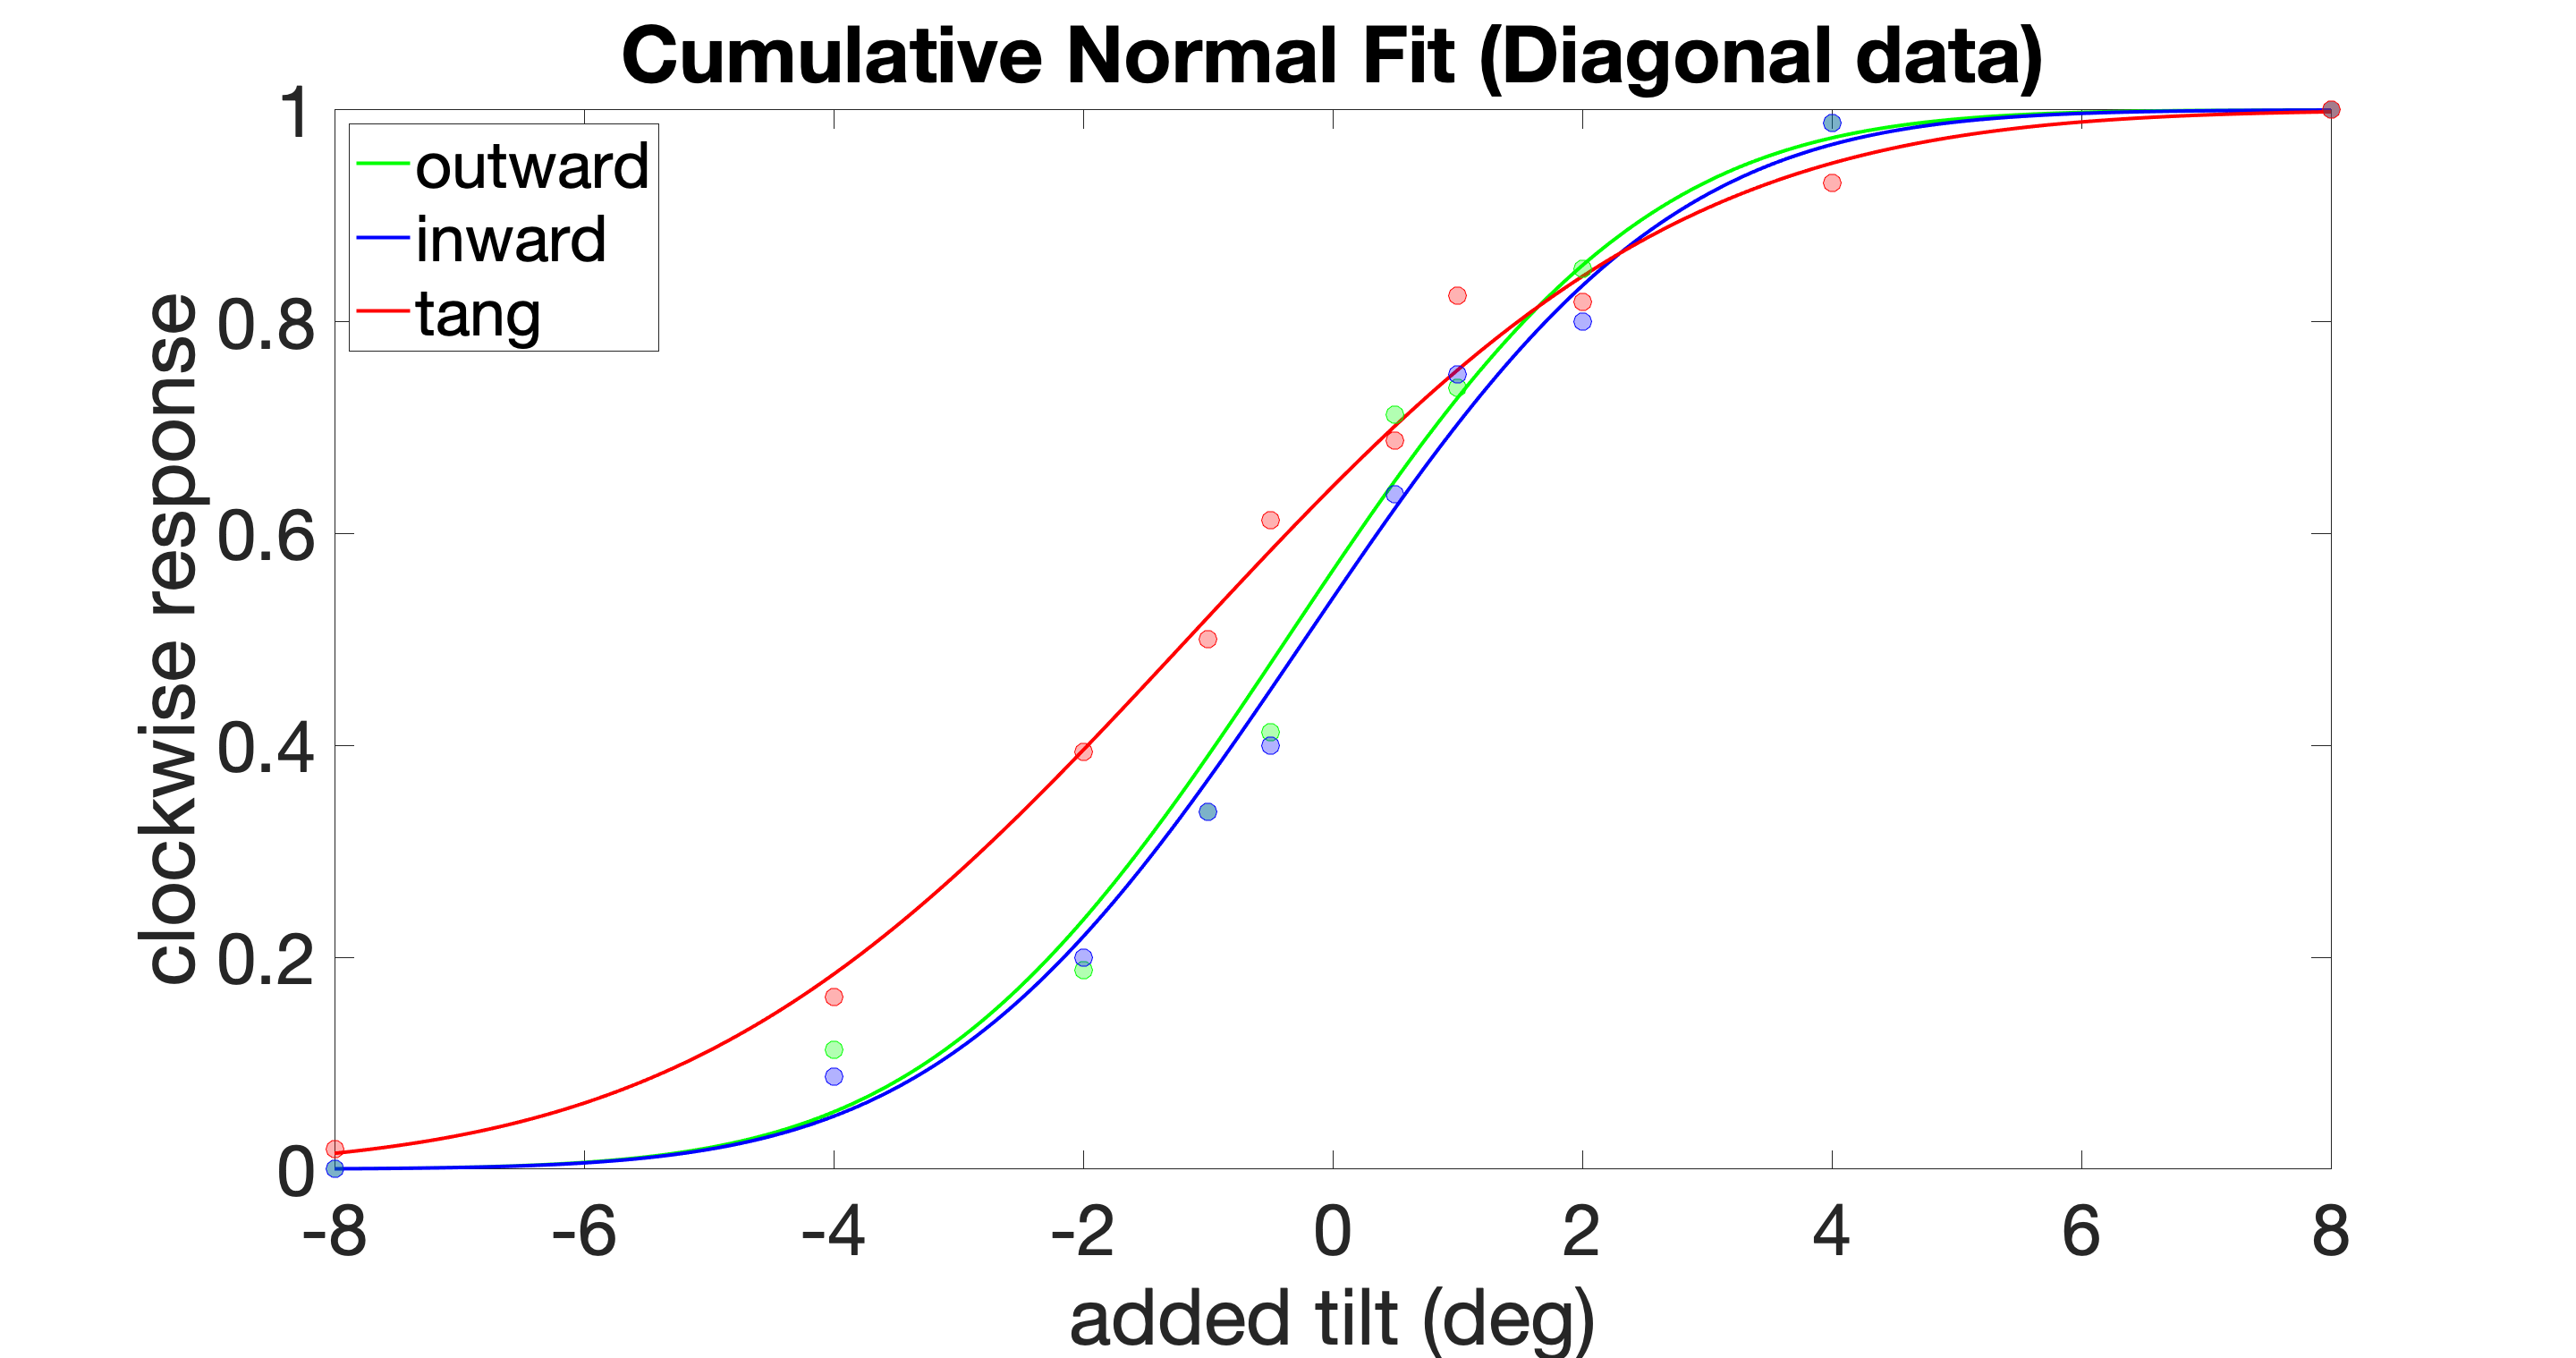
\includegraphics[scale=.06]{Images/PF_obl.png}
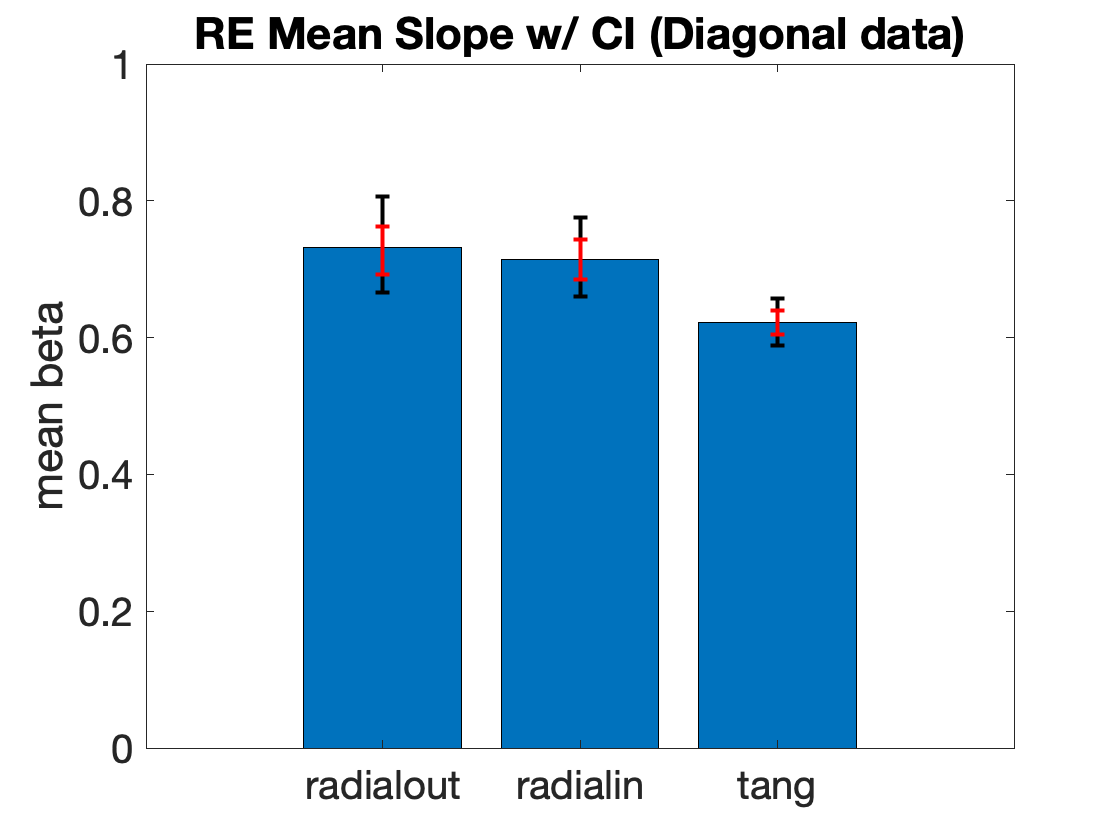
\includegraphics[scale=.11]{Images/MeanSlopeError_obl.png}
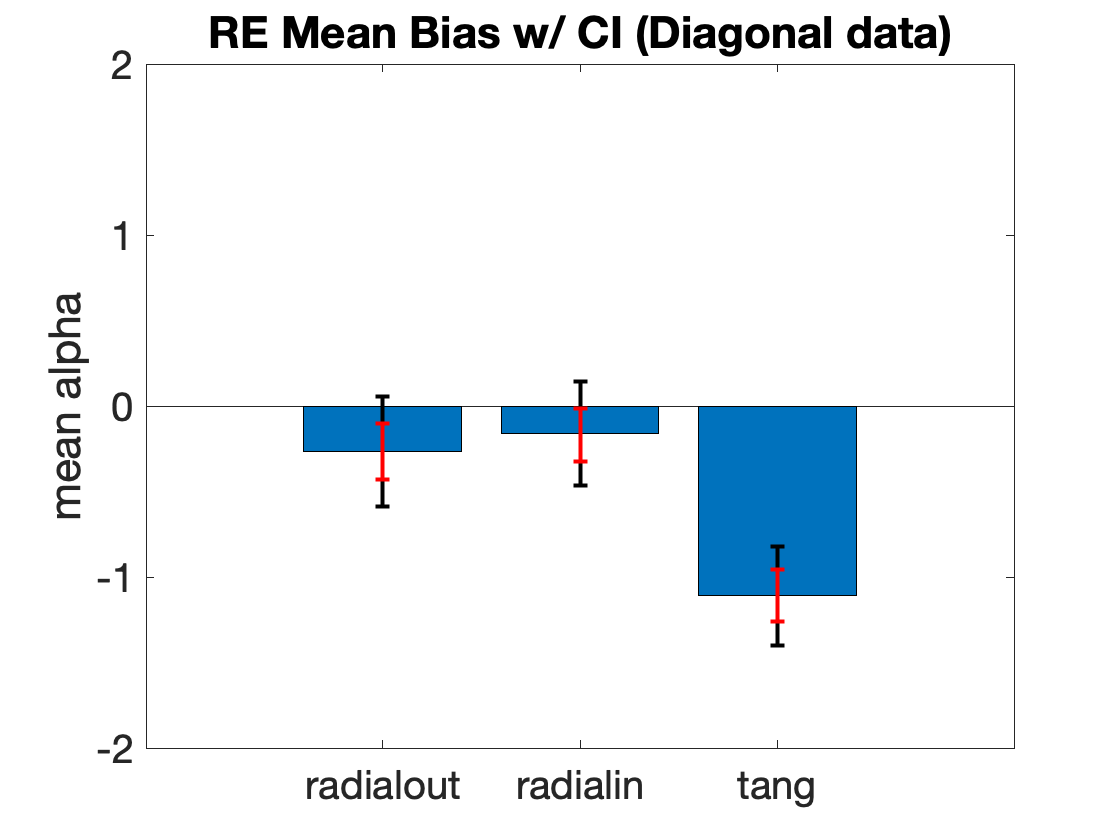
\includegraphics[scale=.11]{Images/MeanBiasError_obl.png}
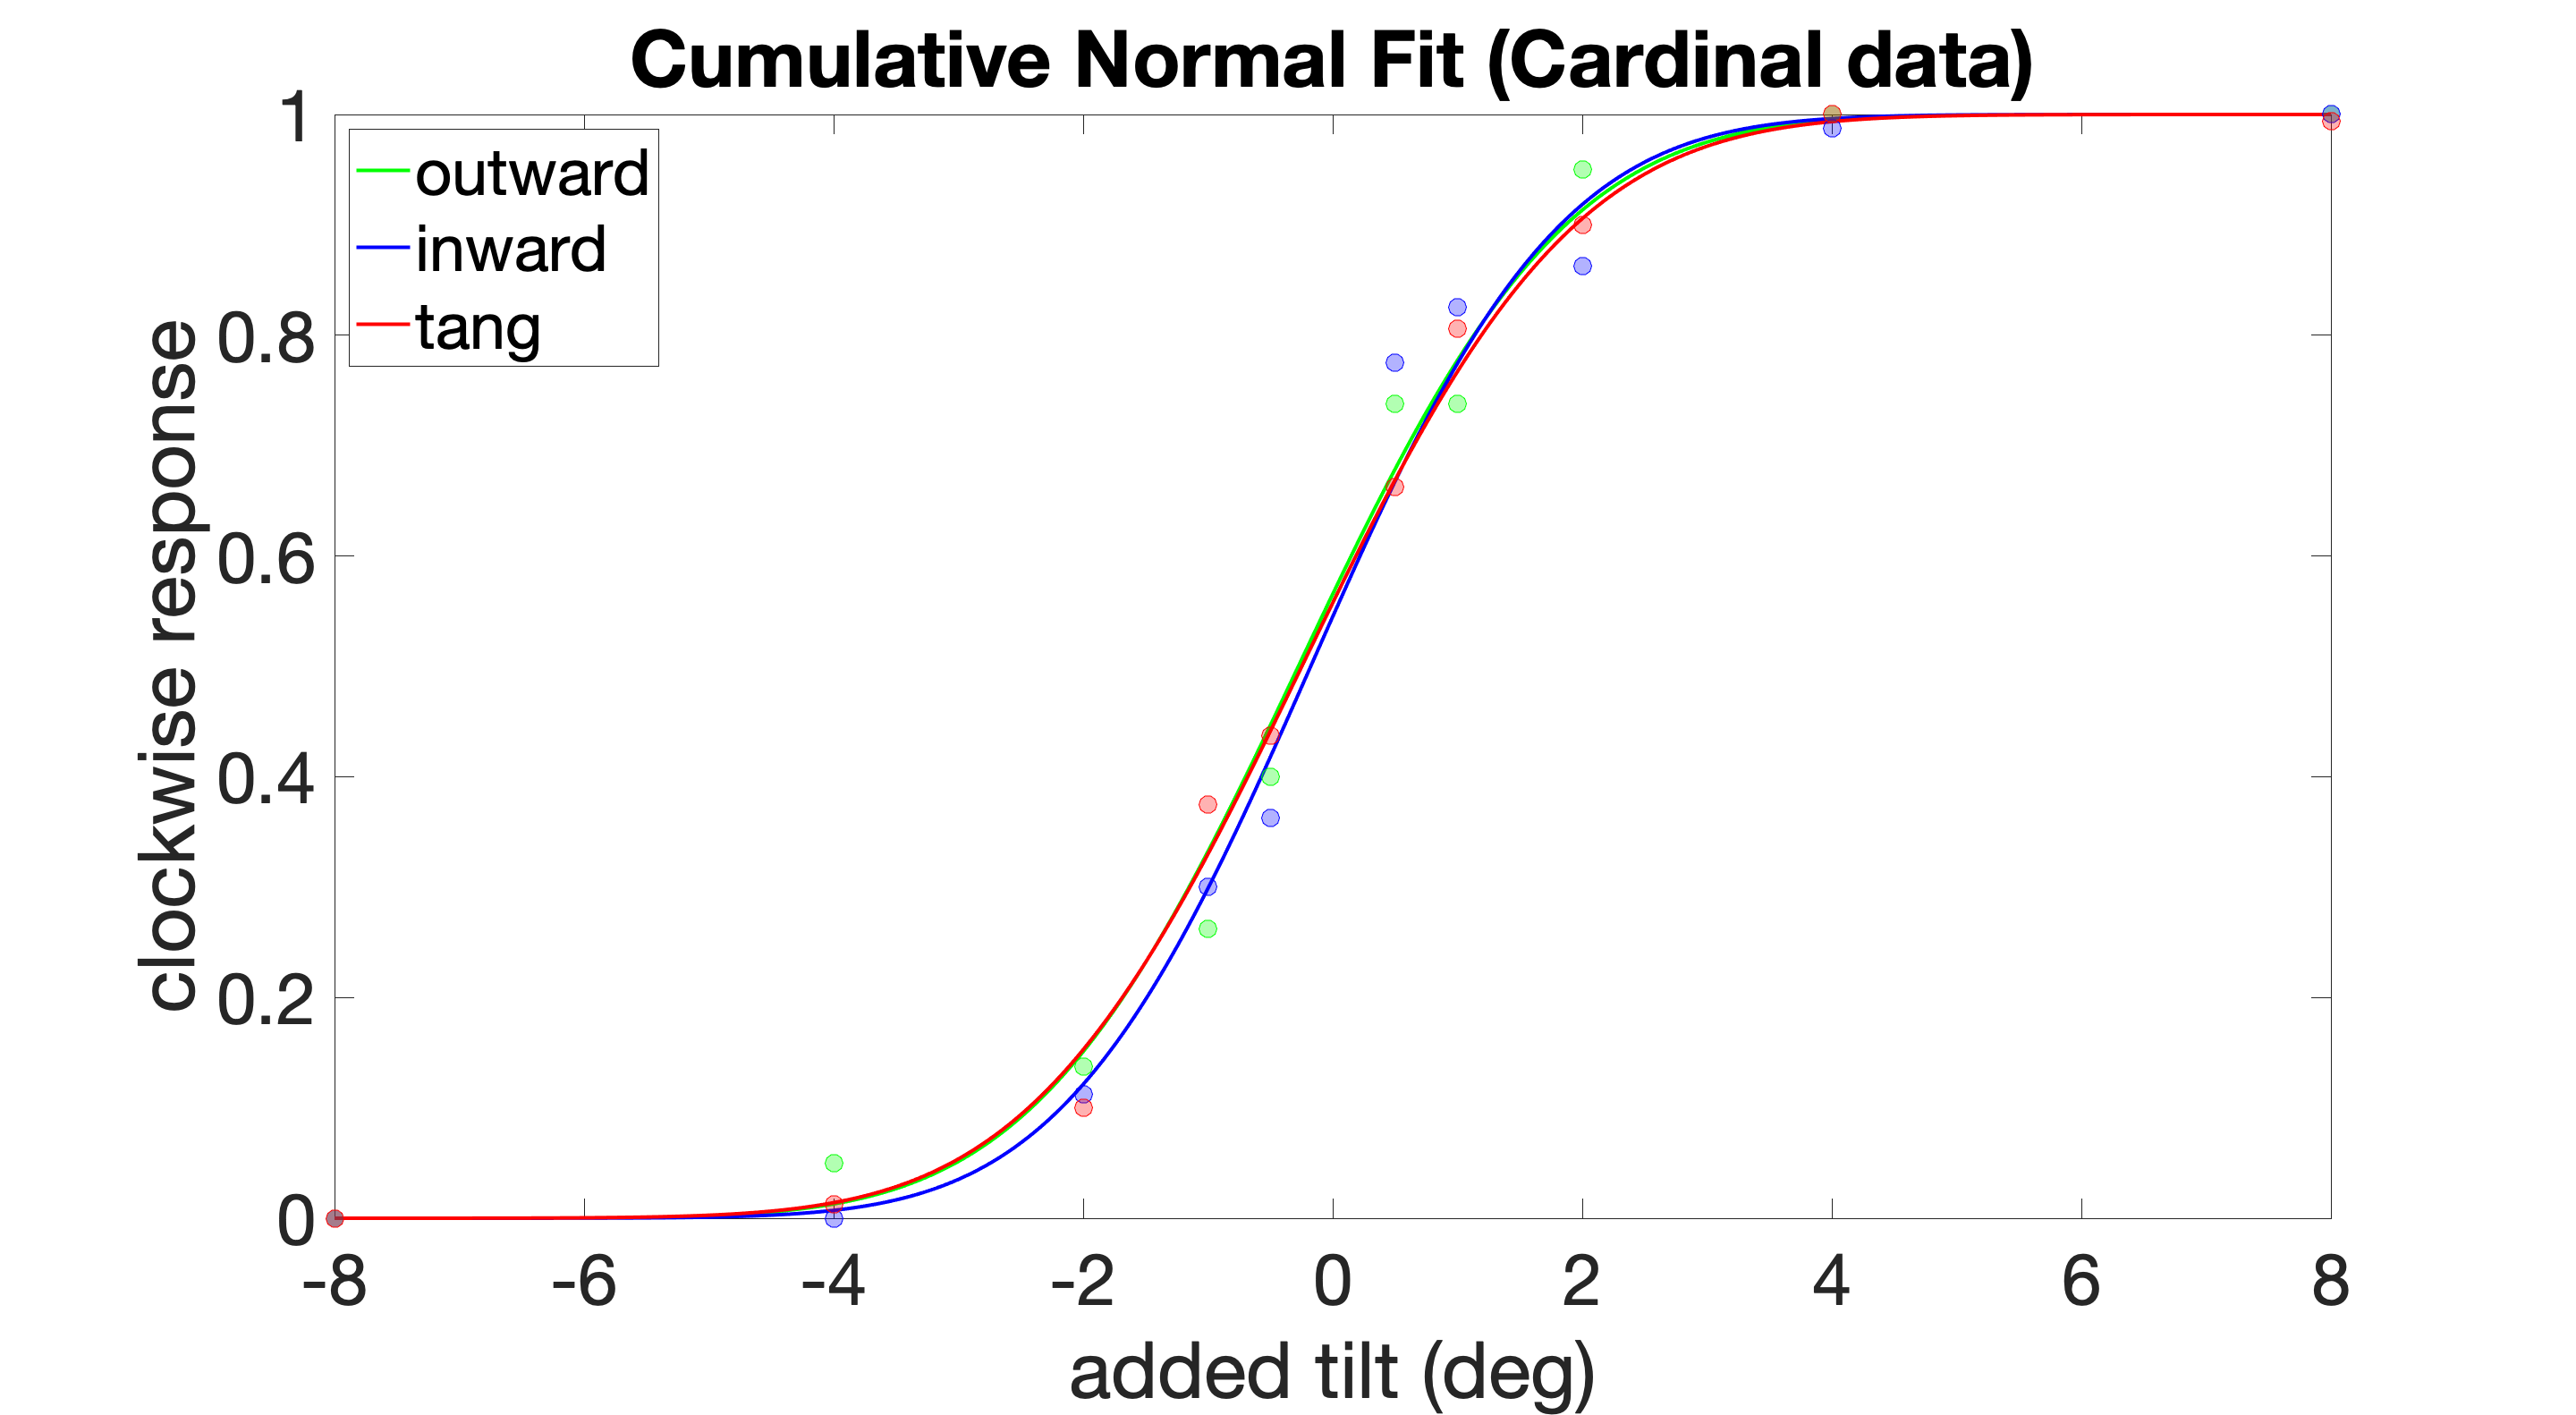
\includegraphics[scale=.06]{Images/PF_card.png}
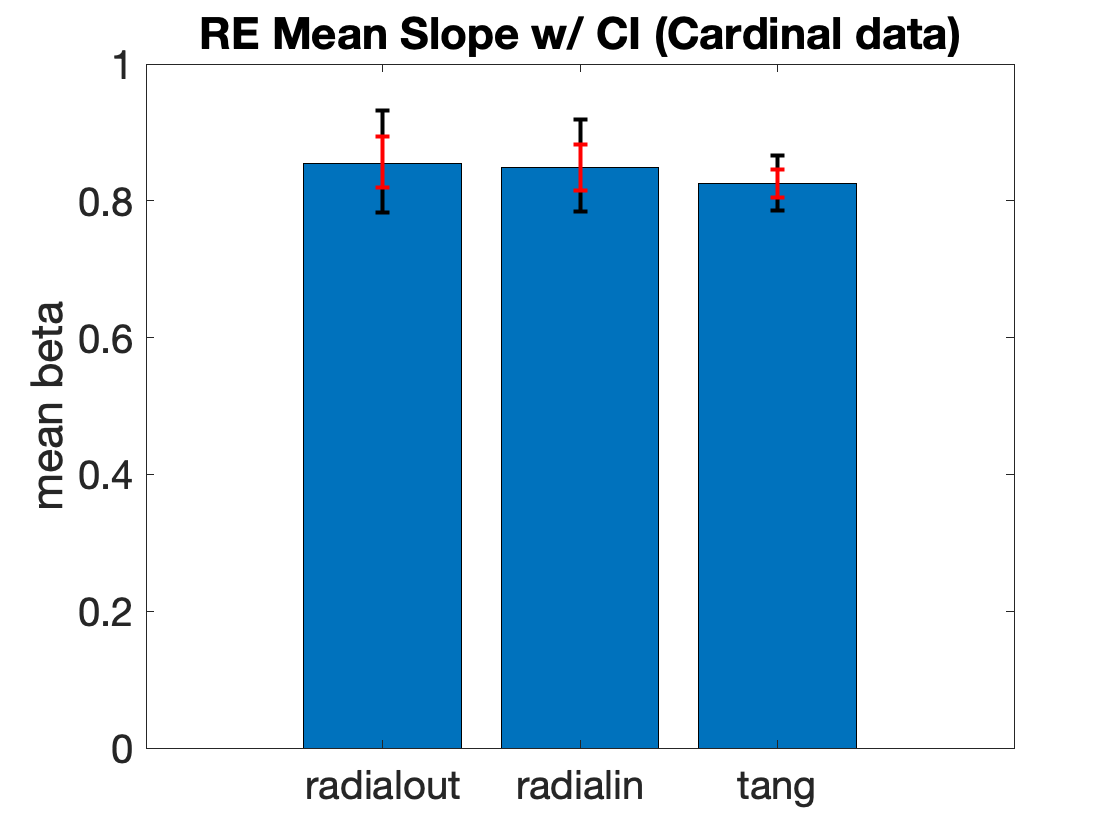
\includegraphics[scale=.11]{Images/MeanSlopeError_card.png}
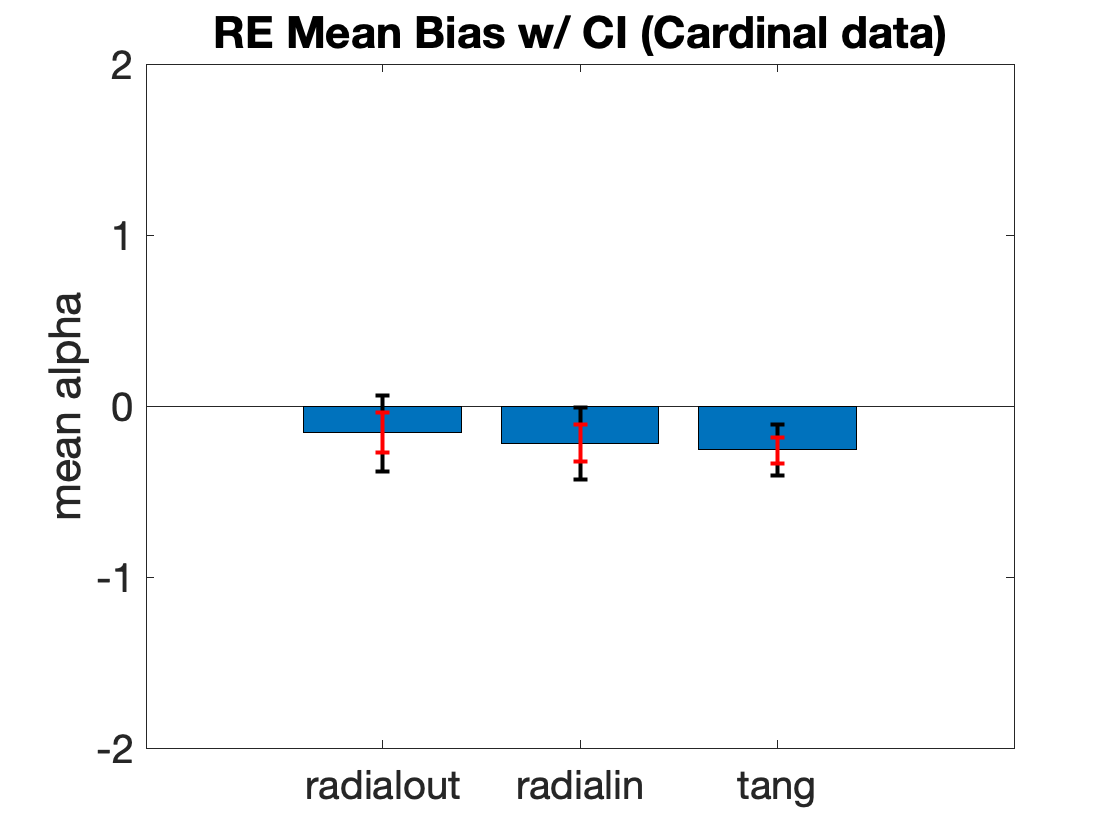
\includegraphics[scale=.11]{Images/MeanBiasError_card.png}
\caption{RE new data (speed 8 cyc/deg) across 8 blocks that each contain 1 reference vector. Top row: All trials (combining cardinal and oblique blocks). Each point = (20 x 8 locations); Second row: subset of data in first row, including only the oblique motion directions (diagonal locations). Each point = (20 x 4 locations); Last row: subset of data in first row, including only the cardinal motion directions (cardinal locations). Each point = (20 x 4 locations). Positive bias = more counterclockwise responses. All means/confidence intervals were computed from samples of posterior distribution using Markov chain Monte Carlo method (from PAL\_PFHB\_fitModel.m) - 5000 samples, 3 chains.}
\end{figure}

\textbf{RE SENSITIVIY/SLOPE}
\\
Radial out beta = [cardinal \& diagonal directions =  0.51, cardinal = 0.6, diagonal = 0.44]
\\
Radial in beta = [cardinal \& diagonal directions =  0.52, cardinal = 0.64, diagonal = 0.44]
\\
Tangential beta = [cardinal \& diagonal directions =  0.4, cardinal = 0.58, diagonal = 0.32]
\\
\textbf{RE BIAS}
\\
Radial out alpha = [cardinal \& diagonal directions =  -0.32, cardinal = -0.28, diagonal = -0.37]
\\
Radial in alpha = [cardinal \& diagonal directions =  -0.21, cardinal = -0.18, diagonal = -0.22]
\\
Tangential alpha = [cardinal \& diagonal directions =  0.67, cardinal = -0.25, diagonal = -1.17]

%% testing SF
\newpage
\section{Data}
\subsection{Psychometric Function (Cumulative normal)}
\begin{figure}[H]
\centering % centers the figure
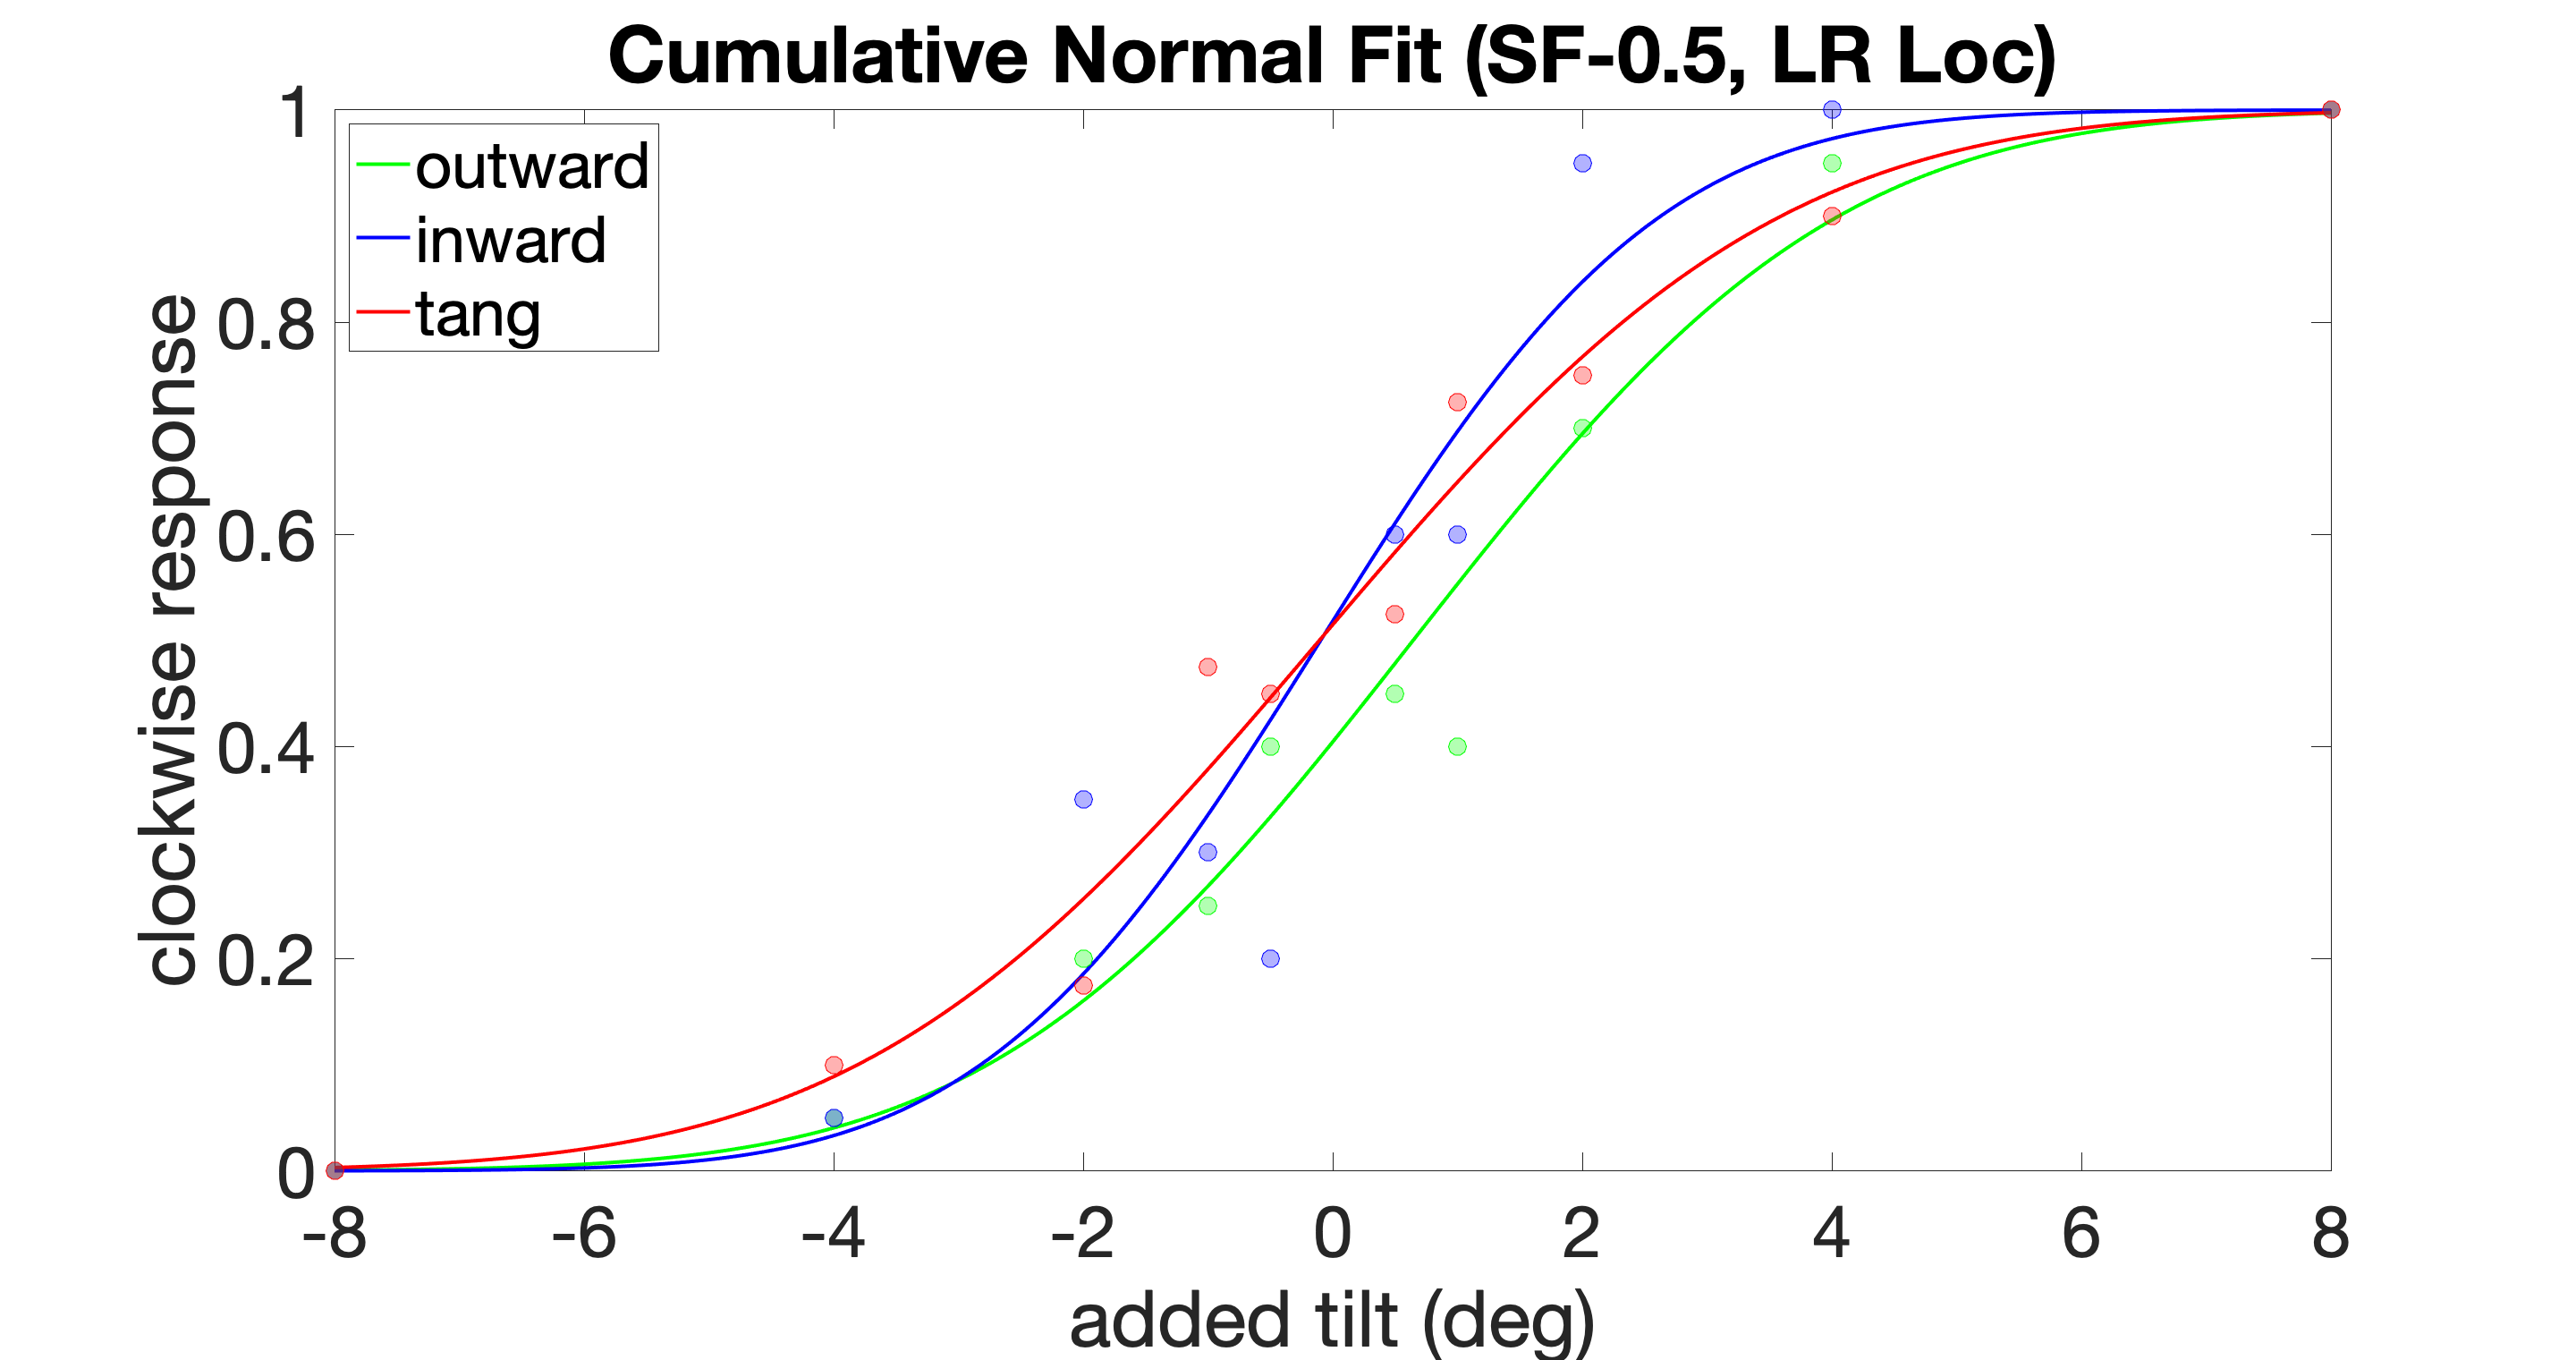
\includegraphics[scale=.06]{Images/PF_SF0.5.png}
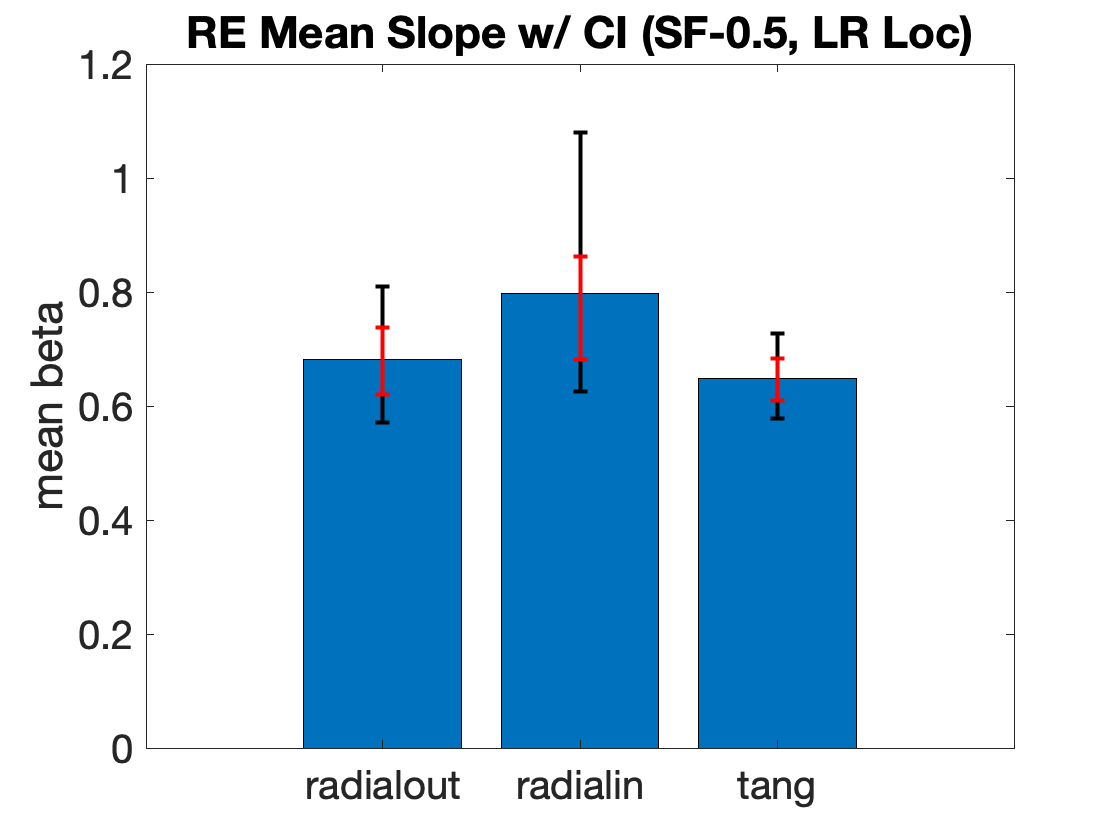
\includegraphics[scale=.11]{Images/MeanSlopeError_SF0.5.png}
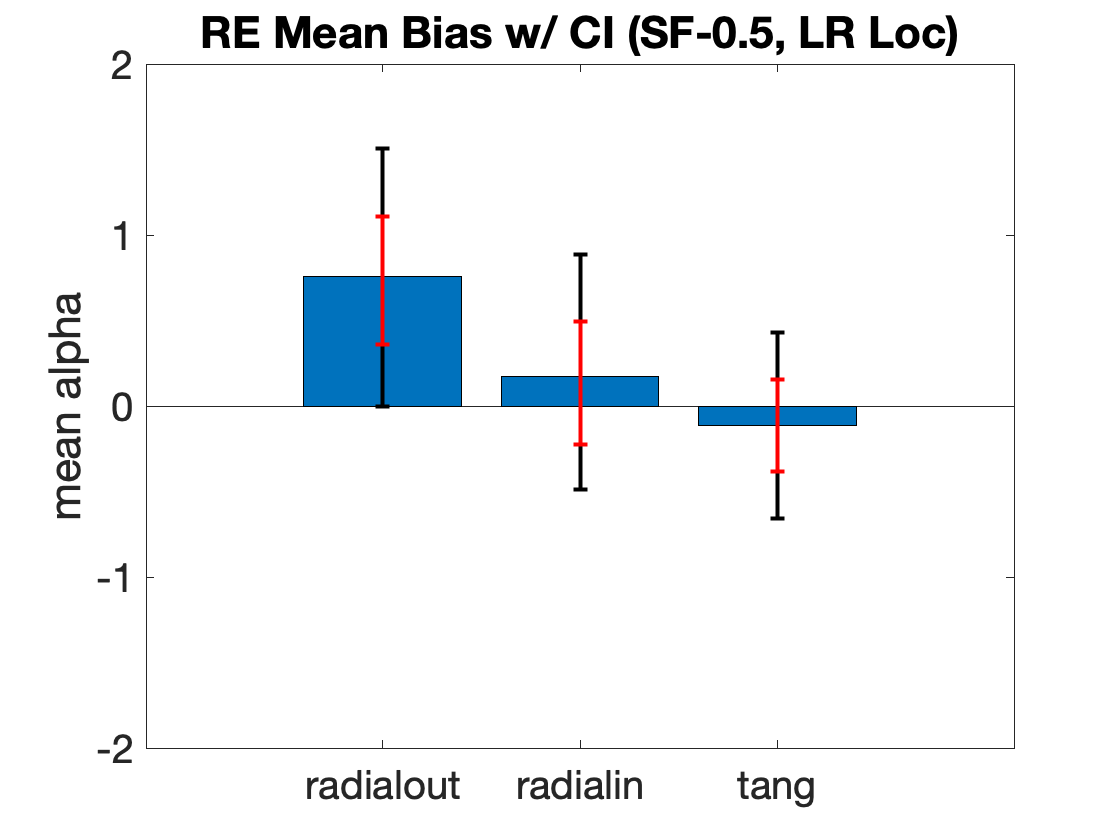
\includegraphics[scale=.11]{Images/MeanBiasError_SF0.5.png}
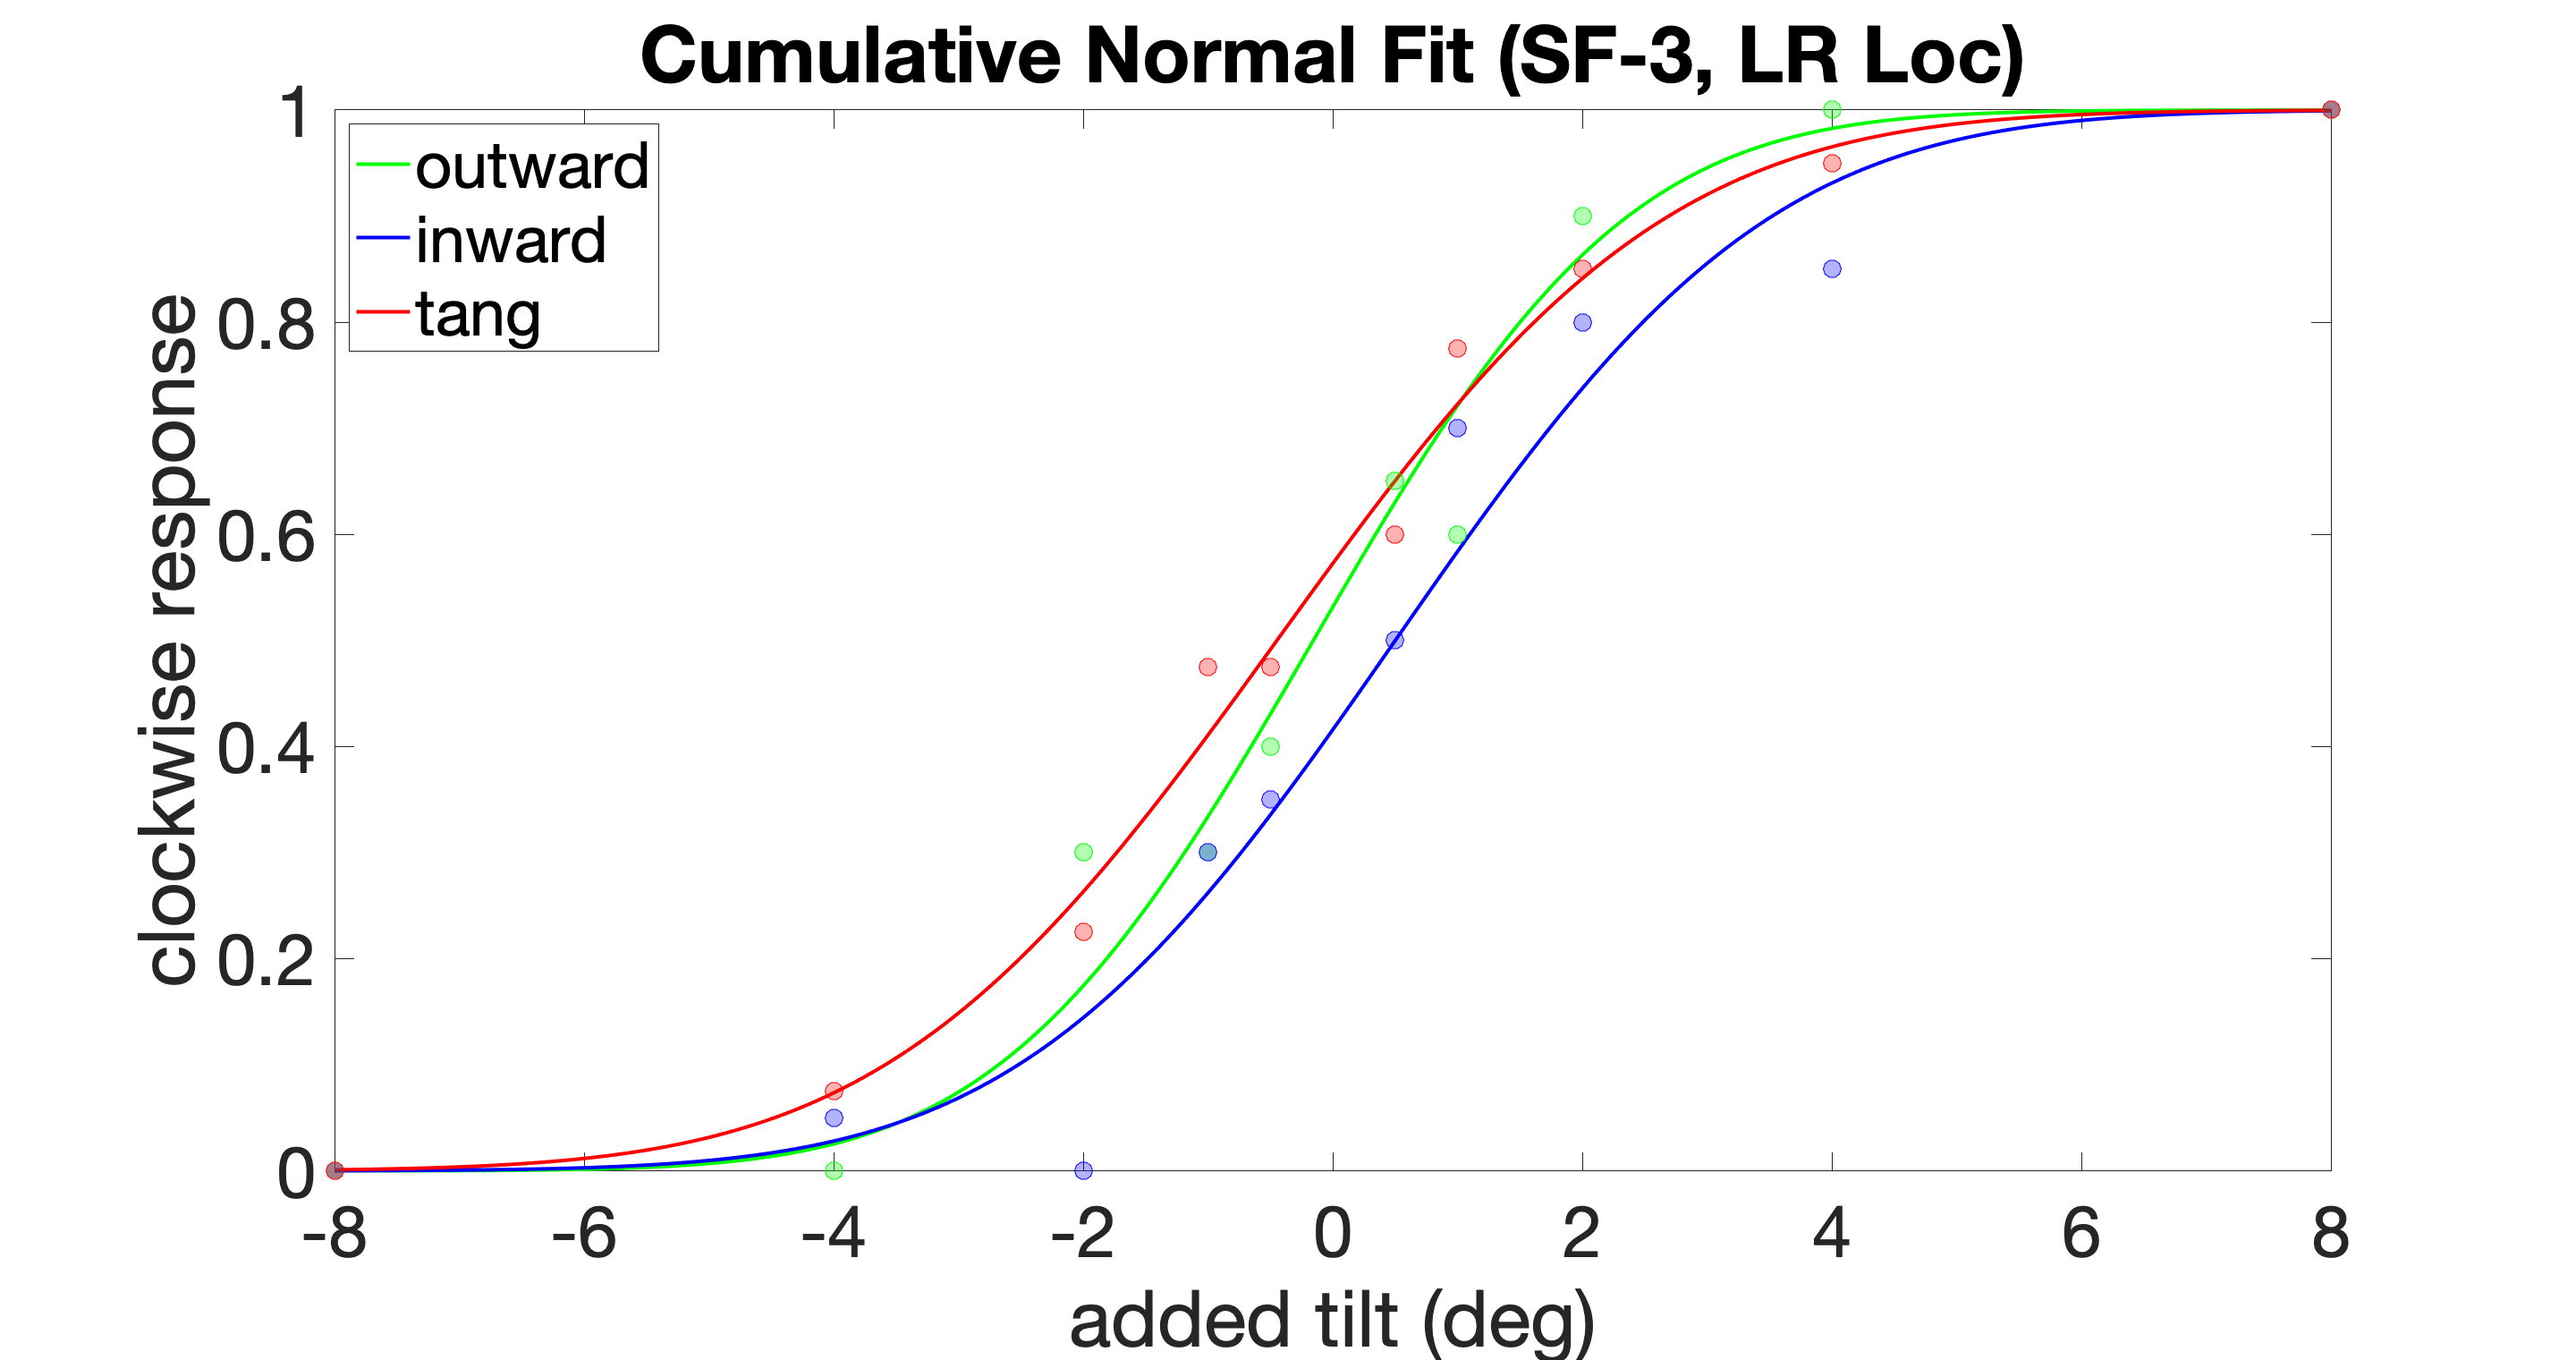
\includegraphics[scale=.06]{Images/PF_SF3.png}
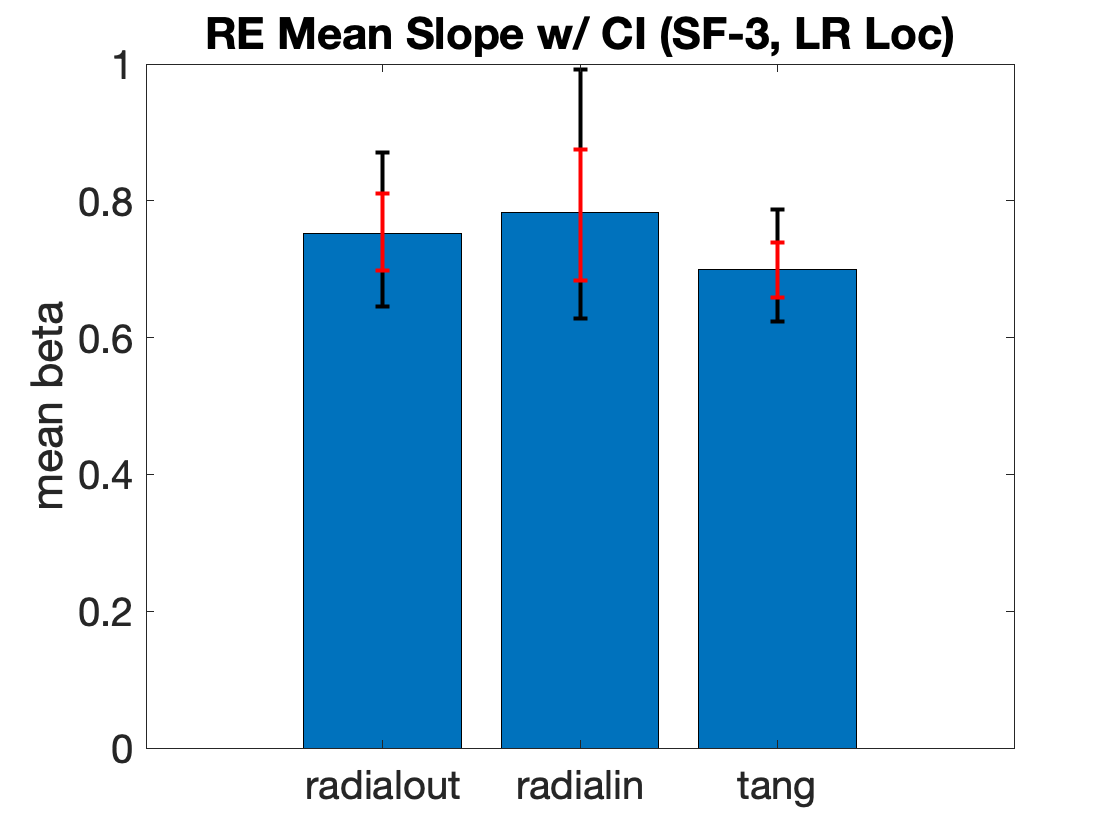
\includegraphics[scale=.11]{Images/MeanSlopeError_SF3.png}
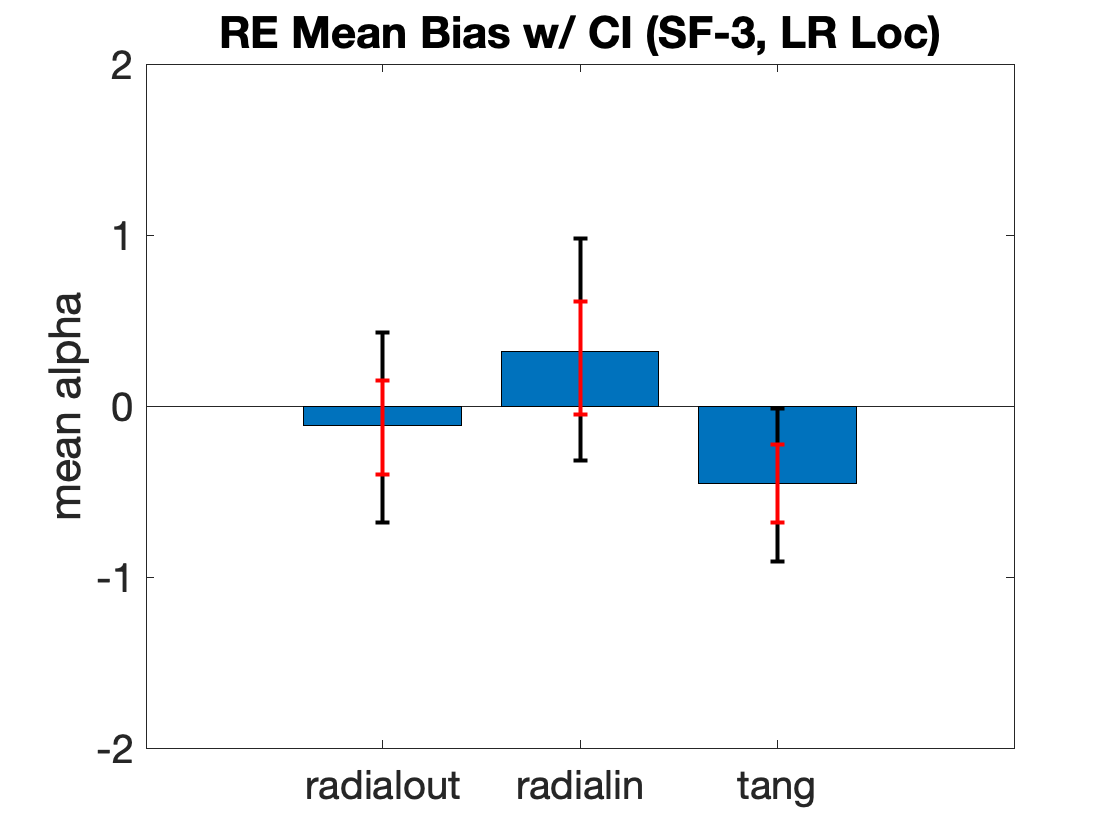
\includegraphics[scale=.11]{Images/MeanBiasError_SF3.png}
\caption{RE new data testing low (SF=0.5) and high (SF=3) spatial frequencies. Only 1 location tested (lower right), which included 200 trials for radialin, 200 for radialout, and 400 tangential.}
\end{figure}

\textbf{RE PERFORMANCE}
\\
Radial out beta = [Low SF = 0.76, High SF = 0.82]
\\
Radial in beta = [Low SF = 0.825, High SF = 0.82]
\\
Tangential beta = [Low SF = 0.77, High SF = 0.79]
\\
\textbf{RE SENSITIVIY/SLOPE}
\\
Radial out beta = [Low SF = 0.38, High SF = 0.5]
\\
Radial in beta = [Low SF = 0.47, High SF = 0.42]
\\
Tangential beta = [Low SF = 0.35, High SF = 0.41]
\\
\textbf{RE BIAS}
\\
Radial out alpha = [Low SF = 0.65, High SF = -0.16]
\\
Radial in alpha = [Low SF = -0.10, High SF = 0.50]
\\
Tangential alpha = [Low SF = -0.12, High SF = -0.45]
%% ^^ Testing SF


\newpage
\subsection{Polar Angle Plot}
\begin{figure}[H]
\centering % centers the figure
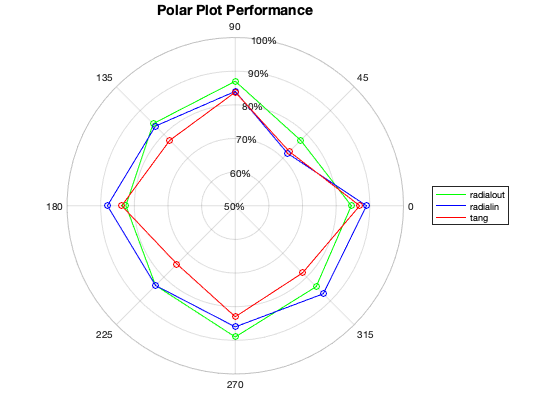
\includegraphics[scale=.5]{Images/performance_polarplot.png}
\caption{Polar plots by performance (range 50-100\%). Each point is 400 trials (collapsed across blocks).}
\end{figure}
\subsection{Quality Control \& Misc.}
\begin{figure}[H]
\centering % centers the figure
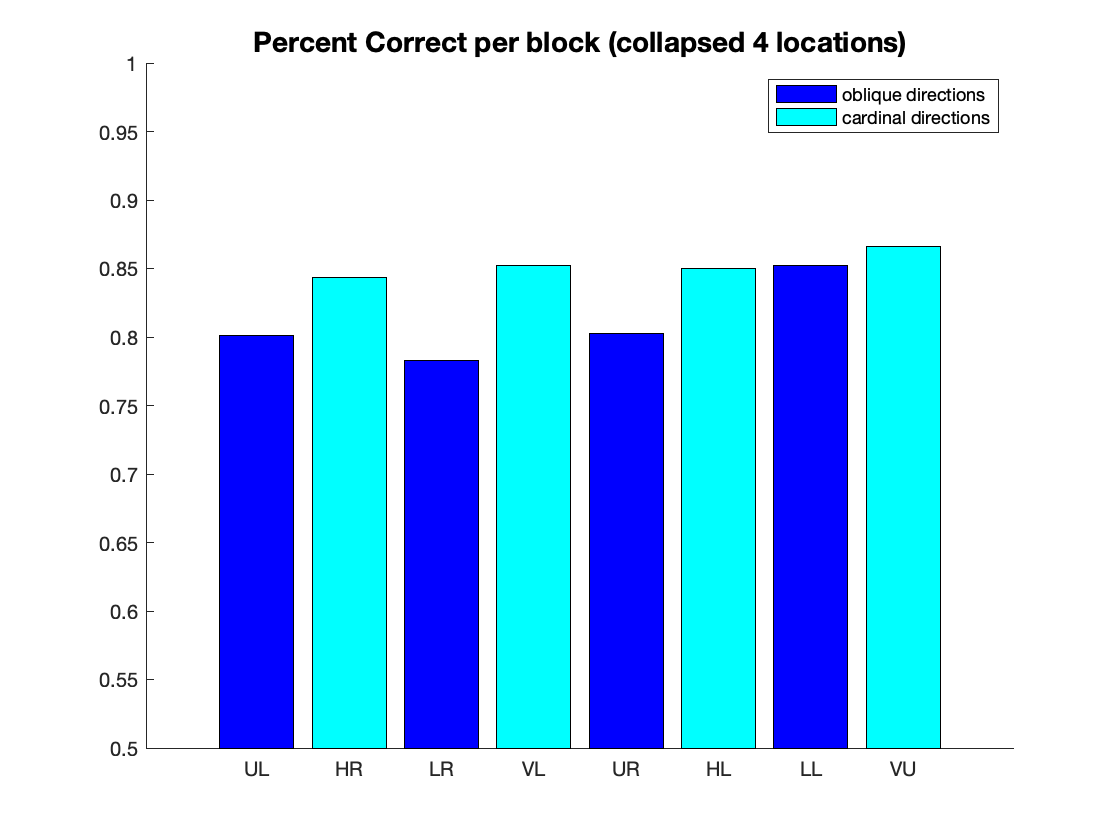
\includegraphics[scale=.25]{Images/block_performance.png}
\caption{To check that performance does not vary too much between blocks. Cardinal blocks are interweaved with diagonal blocks, and consistently show better performance.}
\end{figure}

\newpage
\section{Current Goals} 
\begin{enumerate}
	\item Does radial bias occur in respect to motion direction or orientation of 1D drifting gratings? So far, evidence points to motion direction (but potentially conflicts with Hong paper).
	\item Is there a difference in sensitivity to radial-inward vs. radial-outwards motion? So far, there doesn't seem to be a difference at 7 deg eccentricity.
	\item Does radial bias increase with eccentricity? Within radial condition, does difference of sensitivity between inwards/outwards motion increase with eccentricity?
	\item Is sensitivity to cardinal locations (i.e. orientations/directions) greater than sensitivity to diagonal locations (oblique orientations/directions)? Radial bias and cardinal bias might jointly result in better performance.
	\item Is there an HVA or VMA present at given eccentricities?
	\item How does this extend to plaid stimuli? Does the bias apply to the component motion direction or the apparent motion direction?
\end{enumerate}

\newpage
\section{Updates} 
\begin{itemize}
\item Design Related
	\begin{itemize}
	\item Now running trials using 4 polar angles per block (block 1 = diagonal (e.g. upper left), block 2 = cardinal (upper vertical), block 3 = diagonal (upper left), etc.)
		\begin{itemize}
			\item{Note: For cardinal locations, it feels difficult to not perform task based on orientation}
		\end{itemize}
	\item Implemented log spacing (0.5 - 8) for stimuli for whenever eye tracking.
	\item Same number of trials run for tangential left/right, and radial in/out for balance.
	\end{itemize}
\item Analysis Related
	\begin{itemize}
	\item Changed permanently to higher speed (8 deg / s) and full block runs for all polar angles.
	\item Running 2 spatial frequencies at one location (to test differences)
	\end{itemize}
\item Other improvements
	\begin{itemize}
	\item n/a
	\end{itemize}
\item For discussion
	\begin{itemize}
	\item \textbf{Eye tracker in RM 956}
		\begin{itemize}
			\item{No server connection in that room.}
			\item{Need to calibrate CRT monitor.}
		\end{itemize}
	\item \textbf{Subject payments, grant}
	\item \textbf{Traveling to AD (July?)}
	\item \textbf{VSS expenses}
	\end{itemize}
\end{itemize}

\section{To Do} 
\begin{itemize}
\item Feedback from Feb 17, 2021
	\begin{itemize}
	\item Jon: Re-plot polar angle plot with arrows pointing in direction (length indicating performance)
	\item Difficulty level is good as is, and block design is ok
	\item Collect data with current params for 1-2 subjects w/ eyetracker
	\item If we want to capture polar angle differences, might need to increase SF? (confirmed in other exp around 6 cpd, 6 deg ecc)
	\item Titration for cardinal v. oblique? Or keep the constant stimuli? Dynamic staircase methods?
	\end{itemize}
\item Other
	\begin{itemize}
	\item Use next meeting to go overall plan conceptually (gratings, plaids etc.)
	\item Report sensitivity (d prime) instead of performance
	\item Maybe report reliability? \begin{equation}1/sigma^{2}\end{equation}
	\item Double check sigma of gaussian for reporting purposes (and at what eccentricity contrast drops below 1 perc)
	\end{itemize}
\end{itemize}

\section{Software to Cite}
\begin{itemize}
\item PsychToolbox Extensions (Brainard, 1997; Pelli, 1997; Kleiner et al, 2007)
\item Prins, N \& Kingdom, F. A. A. (2018) Applying the Model-Comparison Approach to Test Specific Research Hypotheses in Psychophysical Research Using the Palamedes Toolbox. Frontiers in Psychology, 9:1250. doi: 10.3389/fpsyg.2018.01250
\item Plummer, M. (2003, March). JAGS: A program for analysis of Bayesian graphical models using Gibbs sampling. In Proceedings of the 3rd international workshop on distributed statistical computing (Vol. 124, No. 125.10, pp. 1-10). (http://mcmc-jags.sourceforge.net/)
\end{itemize}

\end{document}